%% ------------------------------------------------------------------------- %%
\chapter{Introdução}
\label{cap:introducao}


Esse trabalho surge de uma colaboração entre a empresa Intercement e o Laboratório de Lógica, Inteligência Artificial e Métodos Formais do IME-USP. Foram concedidos 10 anos de dados de diversas etapas da produção de cimento do complexo de Cajati, uma das plantas da empresa. Esse trabalho é um estudo com a análise desses dados, desde a sua limpeza até uma criação de modelos preditivos para os mesmos. \\

Os dados são medições de diversos parâmetros em meio ao processo do fabricação do cimento. Eles são divididos em diversas planilhas para diferentes etapas da produção de cimento, são elas, em ordem no processo:

\begin{itemize}
        \item Cimento Cru
        \item Farinha
        \item Clinquér
        \item Produção de Cimento
        \item Expedição
\end{itemize}


Esse trabalho irá aplicar métodos modernos de ML e DP para a modelagem desses dados. Dado que o problema em questão é de \textbf{regressão}, i.e. queremos prever valores numéricos, saímos do domínio canônico onde são aplicados métodos de DL, como por por exemplo NLP ou visão computacional. Nesse trabalho serão reproduzidos modelos propostos por \citet{ubertime} e \citet{energylstm} para problemas de regressão.



%% ------------------------------------------------------------------------- %%
\section{Produção de Cimento}
\label{sec:producao}

Com o fim  

\begin{figure}[H]
\centering
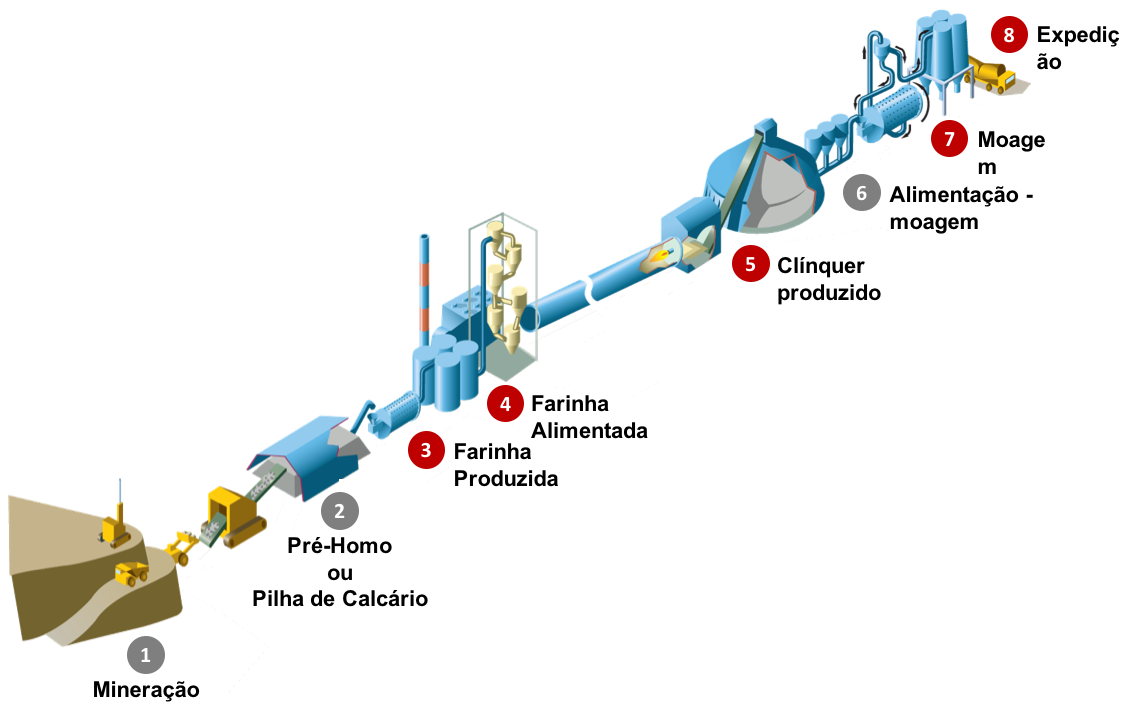
\includegraphics[width=0.9\columnwidth]{cimento.png}
\caption{Representação das Diversas Etapas da produção de Cimento}
\end{figure}


%% ------------------------------------------------------------------------- %%
\section{Objetivos}
\label{sec:objetivo}

Texto texto texto texto texto texto texto texto texto texto texto texto texto
texto texto texto texto texto texto texto texto texto texto texto texto texto
texto texto texto texto texto texto.


%% ------------------------------------------------------------------------- %%
\section{Organização do Trabalho}
\label{sec:organizacao_trabalho}

No Capítulo~\ref{cap:conceitos}, apresentamos os conceitos ... Finalmente, no
Capítulo~\ref{cap:conclusoes} discutimos algumas conclusões obtidas neste
trabalho. Analisamos as vantagens e desvantagens do método proposto ... 

As sequências testadas no trabalho estão disponíveis no Apêndice \ref{ape:sequencias}.
